\chapter{细胞周期调控与程序性细胞死亡}\label{ch:b3:cell-cycle-apoptosis}

你体内约有一千亿个细胞今天会有意死亡，
同样数量的细胞会出生以取而代之；肠道内壁
每五天更新一次，红细胞每四个月更新一次。
蝌蚪失去尾巴时不会出血；人类胚胎的
指间蹼在第八周消失；一个大脑中曾经产生的
神经元中约一半在出生前即被杀死。这些死亡
都由细胞自身按程序执行，每一次
诞生都受一套控制系统许可，该系统在两三个
节点上决定细胞能否继续前进。两套程序
——分裂与自杀——正是本章的主题。它们是
在酵母、蛙卵、海胆以及一种线虫中阐明的，
该线虫恰好有 $1090$ 个体细胞，其中恰好 $131$ 个死亡，二者
在人类中同样适用，其失效一方面导致癌症，
另一方面导致退行性病变。

\section{周期的引擎}

\begin{definition}[细胞周期蛋白与细胞周期蛋白依赖性激酶]\label{def:b3:cell-cycle-apoptosis:cdk}
\index{细胞周期蛋白}\index{细胞周期蛋白依赖性激酶}\index{后期促进复合物}\index{细胞周期}
细胞周期——G1、S（复制）、G2、M（有丝分裂）——由一族蛋白激酶驱动，
即\emph{细胞周期蛋白依赖性激酶}
（CDK），其催化亚基在整个周期中都存在，但只有与
\emph{细胞周期蛋白}结合时才有活性；细胞周期蛋白是一种调节亚基，其浓度按固定顺序升降：
G1 期中，细胞周期蛋白 D 与 Cdk4/6 结合，响应生长因子；
G1/S 转换时，细胞周期蛋白 E 与 Cdk2 结合；
S 期中，细胞周期蛋白 A 与 Cdk2 结合；
进入有丝分裂时，细胞周期蛋白 B 与 Cdk1 结合。每一种复合物都磷酸化其所在时期的蛋白质——
复制起点、核纤层蛋白、凝缩蛋白，以及纺锤体\omterm{def:b3:genomics:assembly}{组装}所需的酶——
每种复合物又因其细胞周期蛋白被降解而失活：
泛素连接酶（G1/S 期为 SCF，有丝分裂期为\emph{后期促进
复合物}，即 APC/C）为细胞周期蛋白加上标签，供蛋白酶体降解。
Cdk1 的活性还受到两种调控：一是由激酶 Wee1 施加、
由磷酸酶 Cdc25 去除的抑制性磷酸化；二是
能结合复合物的小抑制蛋白（p21、p27、p16）。
因此，细胞周期是一系列有序的激酶浪潮，
每一波都以产生它的分子被蛋白水解而结束。
\end{definition}

\begin{proof}[证据]
三条研究线索汇聚到一起。哈特韦尔（20 世纪 70 年代）分离出
出芽酵母的温度敏感型 \emph{cdc} 突变体，每个突变体都停滞在某一阶段，
并具有特征性的芽体大小；他还定义了 \emph{Start}，即 G1 期中
细胞在此之后便确定进入\omterm{def:b3:cell-cycle-apoptosis:cdk}{细胞周期}的时间点。纳斯（20 世纪 80 年代）在裂殖酵母中发现，
\emph{cdc2} 控制有丝分裂的时机，并且
将人类基因导入酵母后，它挽救了突变体：该激酶为
Cdk1，从酵母到人类都是保守的。亨特（1983 年）在海胆卵中发现
一种蛋白质，它在每个周期中逐渐积累，并在每次分裂时
突然被降解，他将其命名为\omterm{def:b3:cell-cycle-apoptosis:cdk}{细胞周期蛋白}。与此同时，蛙卵
中得到了一种“成熟促进因子”，它能驱使任何细胞核
进入有丝分裂；它就是与 Cdk1 结合的\omterm{def:b3:cell-cycle-apoptosis:cdk}{细胞周期蛋白} B。饶和约翰逊
（1970 年）通过融合细胞证明：处于 S 期的细胞能驱使 G1 期
的细胞核进行复制，而 G2 期的细胞核则等待——细胞质携带信号，
而已经复制过的细胞核，
无法被再次诱导复制。
\end{proof}

\begin{omfigure}
\begin{tikzpicture}[every node/.style={font=\scriptsize}, >=stealth]
  % cycle circle with phases
  \draw[very thick, omDef!50] (0,0) circle (2.2);
  \foreach \a/\b/\col/\lab/\r in {90/200/omDef!25/G1/1.55, 200/270/omProp!30/S/1.55, 270/315/omMeth!30/G2/1.55, 315/450/omThm!30/M/1.55} {
    \fill[\col] (0,0) -- (\a:2.2) arc[start angle=\a, end angle=\b, radius=2.2] -- cycle;
    \node[font=\small\bfseries] at ({(\a+\b)/2}:\r) {\lab};
  }
  \fill[white] (0,0) circle (1.0);
  \draw[very thick, omDef!50] (0,0) circle (2.2);
  % cyclin-CDK labels around
  \node[left, align=right] at (-2.4,1.2) {细胞周期蛋白 D--Cdk4/6\\生长因子，Rb 失活};
  \node[left, align=right] at (-2.4,-1.0) {细胞周期蛋白 E--Cdk2\\复制起点启动};
  \node[anchor=north east, align=right] at (-1.3,-2.2) {细胞周期蛋白 A--Cdk2\\复制};
  \node[right, align=left] at (2.4,-1.0) {细胞周期蛋白 B--Cdk1\\进入有丝分裂};
  \node[right, align=left] at (2.4,1.3) {APC/C 降解细胞周期蛋白 B\\和分离酶：后期，退出};
  % checkpoints as bars
  \foreach \a in {160,270,20} \draw[very thick, omThm] (\a:1.95) -- (\a:2.45);
  \node[align=center, anchor=south east] at (-1.2,2.35) {限制点：\\生长因子？};
  \node[align=left, anchor=west] at (2.55,0.35) {纺锤体组装检查点：\\所有动粒是否都已附着？};
  \node[align=center, anchor=north] at (1.5,-2.55) {G2/M 检查点：\\DNA 是否完整？};
  \draw[->, thick] (0,0) ++(60:1.25) arc[start angle=60, end angle=30, radius=1.25];
\end{tikzpicture}

{\small \omterm{def:b3:cell-cycle-apoptosis:cdk}{细胞周期}是一系列\omterm{def:b3:cell-cycle-apoptosis:cdk}{细胞周期蛋白}–CDK 浪潮，每一波都由其\omterm{def:b3:cell-cycle-apoptosis:cdk}{细胞周期蛋白}
的降解而结束；三个\omterm{def:b3:cell-cycle-apoptosis:checkpoints}{检查点}（红色竖条）处，
细胞在此询问是否继续前进。}
\end{omfigure}

\begin{theorem}[开关与延迟制动构成振子]\label{thm:b3:cell-cycle-apoptosis:oscillator}
\index{弛豫振荡}\index{双稳态!细胞周期}\index{滞后现象}
设 $A$ 为\omterm{def:b3:cell-cycle-apoptosis:cdk}{细胞周期蛋白} B–Cdk1 的活性，
$C$ 为\omterm{def:b3:cell-cycle-apoptosis:cdk}{细胞周期蛋白} B 的量。假设：（i）对于固定的 $C$，
$A$ 迅速弛豫到一个稳态，该稳态通过正反馈依赖于 $C$（
活化的 Cdk1 激活其激活剂 Cdc25，并抑制其抑制剂 Wee1），
因此稳态曲线 $A^{*}(C)$ 呈 S 形：
当 $C$ 介于两个阈值 $C_{1} < C_{2}$ 之间时，低态与高态同时存在，
系统停留在其所在的分支上（\emph{\omterm{thm:b3:cell-cycle-apoptosis:oscillator}{滞后现象}}）；（ii）$C$ 缓慢变化，
以恒定速率 $k_{s}$ 合成，
并以速率 $k_{d}A\,C$ 通过 APC/C 降解，而活化的 Cdk1 会在一段延迟之后开启 APC/C。
于是系统不存在稳定稳态，并执行\emph{\omterm{thm:b3:cell-cycle-apoptosis:oscillator}{弛豫振荡}}：$C$ 在低分支上积累，
直至超过 $C_{2}$，$A$ 跃迁至高分支（进入有丝分裂）；
降解速率超过合成速率，$C$ 下降，直至低于 $C_{1}$，
$A$ 崩塌回低分支（有丝分裂退出），循环往复。
周期主要由慢变量决定：
上升阶段约为 $C_{2}/k_{s}$，
再加上从 $C_{2}$ 降解至 $C_{1}$ 所需的时间。
\end{theorem}
\begin{proof}[部分证明]
该二元系统的稳态要求 $\mathrm{d}C/\mathrm{d}t = 0$，
即 $k_{s} = k_{d}A^{*}(C)\,C$，位于 S 形曲线上的某一点。
在低分支上 $A^{*}$ 很小，因此有 $k_{d}A^{*}C < k_{s}$，
对于 $C$ 直至 $C_{2}$：\omterm{def:b3:cell-cycle-apoptosis:cdk}{细胞周期蛋白}上升，系统被推离该分支的末端。
在高分支上 $A^{*}$ 很大，因此有 $k_{d}A^{*}C > k_{s}$，
对于 $C$ 下降至 $C_{1}$：\omterm{def:b3:cell-cycle-apoptosis:cdk}{细胞周期蛋白}下降，系统被推离另一端。
唯一可能的稳态将位于中间的不稳定分支上，
而该分支上的点是排斥的；因此不存在稳定稳态，
轨线被限制在两个稳定分支及其间的跳跃之中，
于是循环往复。低分支上的时间为
$\int \mathrm{d}C/(k_{s} - k_{d}A^{*}C) \approx C_{2}/k_{s}$，
此时 $A^{*}$ 很小；而高分支上的时间为
降解 $C_{2} - C_{1}$ 所需的较短时间，速率为 $k_{d}A^{*}_{\text{高}}C$。
Cdc25/Wee1 反馈所导致的 S 形曲线的存在，
此处不加证明地承认；它与本科二年级分册中的
自激活基因属于同一种双稳态，只是此时快变量为一种激酶，
慢变量则为其\omterm{def:b3:cell-cycle-apoptosis:cdk}{细胞周期蛋白}。
\end{proof}

\begin{omfigure}
\begin{tikzpicture}
\begin{axis}[
  width=6.6cm, height=5.6cm,
  axis lines=left,
  xmin=0, xmax=1.4, ymin=0, ymax=1.1,
  xlabel={周期蛋白 B，$C$}, ylabel={Cdk1 活性，$A$},
  xlabel style={font=\small, at={(axis description cs:0.5,-0.12)}, anchor=north}, ylabel style={font=\small},
  tick label style={font=\scriptsize}, xtick={0.4,1.0}, xticklabels={$C_{1}$,$C_{2}$}, ytick=\empty,
  clip=false,
]
% S-shaped nullcline: two stable branches and a dashed unstable one
\addplot[very thick, omDef, smooth] coordinates {(0,0.02) (0.5,0.04) (0.9,0.07) (1.0,0.1)};
\addplot[very thick, omDef, dashed, smooth] coordinates {(1.0,0.1) (0.85,0.3) (0.7,0.5) (0.55,0.7) (0.4,0.9)};
\addplot[very thick, omDef, smooth] coordinates {(0.4,0.9) (0.6,0.94) (1.0,0.97) (1.4,0.98)};
\draw[->, very thick, omThm] (axis cs:0.05,0.15) -- (axis cs:0.98,0.15);
\draw[->, very thick, omThm] (axis cs:1.04,0.18) -- (axis cs:1.04,0.82);
\draw[->, very thick, omThm] (axis cs:0.98,0.84) -- (axis cs:0.42,0.84);
\draw[->, very thick, omThm] (axis cs:0.36,0.82) -- (axis cs:0.36,0.18);
\node[font=\scriptsize, omThm, anchor=south west] at (axis cs:0.36,0.24) {周期蛋白积累};
\node[font=\scriptsize, omThm, anchor=west] at (axis cs:1.07,0.5) {进入};
\node[font=\scriptsize, omThm, anchor=south] at (axis cs:0.7,1.0) {APC/C 降解周期蛋白（有丝分裂）};
\node[font=\scriptsize, omThm, anchor=east] at (axis cs:0.33,0.5) {退出};
\node[font=\scriptsize, omDef, anchor=north east] at (axis cs:1.38,0.95) {$A^{*}(C)$};
\end{axis}
\begin{axis}[
  at={(7.6cm,0)}, anchor=south west,
  width=6.6cm, height=5.6cm,
  axis lines=left,
  xmin=0, xmax=3, ymin=0, ymax=1.2,
  xlabel={时间（周期）}, ylabel={},
  xlabel style={font=\small, at={(axis description cs:0.5,-0.12)}, anchor=north},
  tick label style={font=\scriptsize}, xtick={0,1,2,3}, ytick=\empty,
  clip=false,
]
\addplot[very thick, omDef] coordinates {(0,0.4) (0.8,1.0) (0.95,0.4) (1.75,1.0) (1.9,0.4) (2.7,1.0) (2.85,0.4) (3,0.5)};
\addplot[very thick, omThm] coordinates {(0,0.05) (0.8,0.05) (0.8,0.95) (0.95,0.95) (0.95,0.05) (1.75,0.05) (1.75,0.95) (1.9,0.95) (1.9,0.05) (2.7,0.05) (2.7,0.95) (2.85,0.95) (2.85,0.05) (3,0.05)};
\node[font=\scriptsize, omDef, anchor=south west] at (axis cs:1.0,0.1) {周期蛋白 B};
\node[font=\scriptsize, omThm, anchor=south west] at (axis cs:1.0,1.0) {Cdk1 活性};
\end{axis}
\end{tikzpicture}

{\small 左：振荡器的相平面。S 形曲线
是各周期蛋白水平下 Cdk1 的快稳态；红色环线
即周期——沿低分支缓慢积累，
在 $C_{2}$ 处跳变，沿高分支快速降解，
$C_{1}$ 处跳回。右：由此得到的时间进程，周期蛋白呈锯齿形，
激酶活性呈方波形。}
\end{omfigure}

\begin{example}[蛙卵为何是一个时钟]\label{ex:b3:cell-cycle-apoptosis:frog}
受精的蛙卵在六小时内分裂十二次，
期间无生长、无转录，也没有\omterm{def:b3:cell-cycle-apoptosis:checkpoints}{检查点}，
间隔 \qty{30}{min}：这正是定理中振荡器的裸跑，而
取自其细胞质的提取物在试管中仍持续循环，周期蛋白
反复升降，却无物可分裂。加入不可降解的周期蛋白 B，
提取物便被锁定于有丝分裂期，因为 $C$ 永远不会低于 $C_{1}$；
若阻断周期蛋白的合成，则将其锁定于间期。在体细胞中，
同一引擎外包裹着下一节的调控机制，这些机制将其
停在阈值处，直到条件满足，使周期
变为一天而非半小时，甚至可以无限长。
\end{example}

\section{检查点}

\begin{definition}[检查点]\label{def:b3:cell-cycle-apoptosis:checkpoints}
\index{检查点}\index{限制点}\index{纺锤体组装检查点}\index{复制许可}
称\emph{检查点}为在某一转换处暂停周期的调控，
直到某一条件满足为止，通过作用于引擎本身——抑制
某个 CDK 或泛素连接酶。其中三种最为重要。\emph{限制
点}位于 G1 晚期（酵母中为 Start）：细胞只有在
生长因子、营养物质和细胞大小允许时才继续推进；越过此点后，周期
即使没有它们也会完成。\emph{G2/M 检查点}：受损或未复制的 DNA，
经由\cref{ch:b3:dna-repair}中的 \omterm{def:b3:dna-repair:ddr}{ATM}/ATR 激酶传递信号，使
Cdc25 受抑制，从而 Cdk1 保持磷酸化而失活。
\emph{纺锤体\omterm{def:b3:genomics:assembly}{组装}检查点}：单个动粒未附着于
\omterm{def:b3:cytoskeleton-motility:filaments}{微管}，便会产生一种可扩散的抑制物（与 Cdc20 结合的 Mad2），
它使 APC/C 保持关闭，使后期等待最后一
条染色体就位。第四种调控没有等待步骤，却同样
严格：\emph{复制许可}。复制起点装载 MCM
解旋酶，仅在 G1 期进行（此时 CDK 活性低），装载因子
则在 S 期开始后被破坏或抑制，使每个起点
在每个周期中只启动一次——这正是拉奥与约翰逊的融合实验中 G2 期细胞核
无法被诱导复制的原因。
\end{definition}

\begin{proposition}[限制点是一个开关]\label{prop:b3:cell-cycle-apoptosis:rb}
\index{视网膜母细胞瘤蛋白}\index{E2F}
在 G1 早期，转录因子\emph{\omterm{prop:b3:cell-cycle-apoptosis:rb}{E2F}}驱动 S 期
的基因（周期蛋白 E、周期蛋白 A 和复制酶），其活性
被\emph{\omterm{prop:b3:cell-cycle-apoptosis:rb}{视网膜母细胞瘤蛋白}}Rb 抑制，保持失活。生长因子诱导
周期蛋白 D，周期蛋白 D--Cdk4/6 开始磷酸化 Rb，释放
少量 \omterm{prop:b3:cell-cycle-apoptosis:rb}{E2F}；随后 \omterm{prop:b3:cell-cycle-apoptosis:rb}{E2F} 诱导周期蛋白 E，周期蛋白 E--Cdk2 磷酸化
Rb 的磷酸化大大加强——这是一种正反馈，一旦越过阈值，
无需更多生长因子即可自行完成。细胞已越过
\omterm{def:b3:cell-cycle-apoptosis:checkpoints}{限制点}；\omterm{prop:b3:cell-cycle-apoptosis:rb}{E2F} 还会诱导自身基因。Rb 缺失，或
Cdk4/6 抑制剂 p16 缺失，或周期蛋白 D 扩增，
便彻底消除对生长因子的需求，这些情形在
癌症中很常见（\cref{ch:b3:cancer-biology}）；抑制 Cdk4/6 的药物目前
已用于治疗依赖这一开关的乳腺癌。
\end{proposition}

\begin{omfigure}
\begin{tikzpicture}[every node/.style={font=\scriptsize}, >=stealth]
  \node[draw, thick, rounded corners, fill=omProp!25, minimum width=2.2cm] (gf) at (0,2.2) {生长因子};
  \node[draw, thick, rounded corners, fill=omDef!20, minimum width=2.4cm] (cd) at (0,1.0) {周期蛋白 D--Cdk4/6};
  \node[draw, thick, rounded corners, fill=omThm!20, minimum width=1.6cm] (rb) at (3.8,1.0) {Rb};
  \node[draw, thick, rounded corners, fill=omMeth!25, minimum width=1.6cm] (e2f) at (7.2,1.0) {E2F};
  \node[draw, thick, rounded corners, fill=omDef!20, minimum width=2.4cm] (ce) at (7.2,-0.6) {周期蛋白 E--Cdk2};
  \node[draw, thick, rounded corners, fill=gray!15, align=center, minimum width=2.6cm] (s) at (10.8,1.0) {S 期基因：\\周期蛋白 A、MCM、\dots};
  \draw[->, thick] (gf) -- (cd);
  \draw[-|, thick, omThm] (cd) -- (rb) node[midway, above, font=\tiny] {磷酸化};
  \draw[-|, thick, omThm] (rb) -- (e2f) node[midway, above, font=\tiny] {保持失活};
  \draw[->, thick] (e2f) -- (s);
  \draw[->, thick] (e2f) -- (ce) node[midway, right] {诱导};
  \draw[-|, thick, omThm] (ce.west) -- ++(-2.2,0) |- (rb.south) node[pos=0.25, below] {进一步磷酸化 Rb};
  \draw[->, thick, omMeth!70!black] (e2f.north) .. controls (6.0,2.2) and (6.8,2.2) .. (e2f.north east) node[pos=0.5, above] {诱导自身基因};
  \node[draw, thick, rounded corners, fill=omThm!10] (p16) at (0,-0.6) {p16}; \draw[-|, thick, omThm] (p16) -- (cd);
\end{tikzpicture}

{\small \omterm{def:b3:cell-cycle-apoptosis:checkpoints}{限制点}。生长因子启动 Rb 的磷酸化
使少量 \omterm{prop:b3:cell-cycle-apoptosis:rb}{E2F} 释放；\omterm{prop:b3:cell-cycle-apoptosis:rb}{E2F} 诱导周期蛋白 E，其激酶
进一步磷酸化 Rb——这是一种正反馈，完成这一
转换，使其不再依赖最初的信号。截线
表示抑制。}
\end{omfigure}

\begin{proposition}[后期是一项蛋白水解决定]\label{prop:b3:cell-cycle-apoptosis:anaphase}
\index{分离酶抑制蛋白}\index{分离酶}\index{黏连蛋白}
姐妹染色单体自 S 期起即由环状的
\emph{\omterm{prop:b3:cell-cycle-apoptosis:anaphase}{黏连蛋白}}环维系在一起。中期时，当每个动粒都已附着且
纺锤体\omterm{def:b3:cell-cycle-apoptosis:checkpoints}{检查点}已关闭，APC/C 与其激活因子 Cdc20
使两种蛋白泛素化：周期蛋白 B，其降解使 Cdk1 失活，并
允许细胞退出有丝分裂；以及\emph{\omterm{prop:b3:cell-cycle-apoptosis:anaphase}{分离酶抑制蛋白}}，其降解释放
蛋白酶\emph{\omterm{prop:b3:cell-cycle-apoptosis:anaphase}{分离酶}}，它切割\omterm{prop:b3:cell-cycle-apoptosis:anaphase}{黏连蛋白}。所有姐妹染色单体对
在数秒之内相继分离，被纺锤体拉向两极，并
由肌动蛋白与\omterm{def:b3:cytoskeleton-motility:motors}{肌球蛋白}~II \omterm{def:b3:genomics:assembly}{组装}成的收缩环分裂，该环\omterm{def:b3:genomics:assembly}{组装}于
纺锤体中区向皮层发出信号之处（通过 RhoA）。这一决定是
不可逆的，因为它是蛋白水解的：被切断的\omterm{prop:b3:cell-cycle-apoptosis:anaphase}{黏连蛋白}无法
重新\omterm{def:b3:genomics:assembly}{组装}，被降解的周期蛋白必须重新合成。错误
在此——染色体被拉向错误的极，或后期在最后一个附着完成之前
便开始——会产生非整倍体子细胞，这是
肿瘤和流产中最常见的染色体异常。
\end{proposition}

\begin{omfigure}
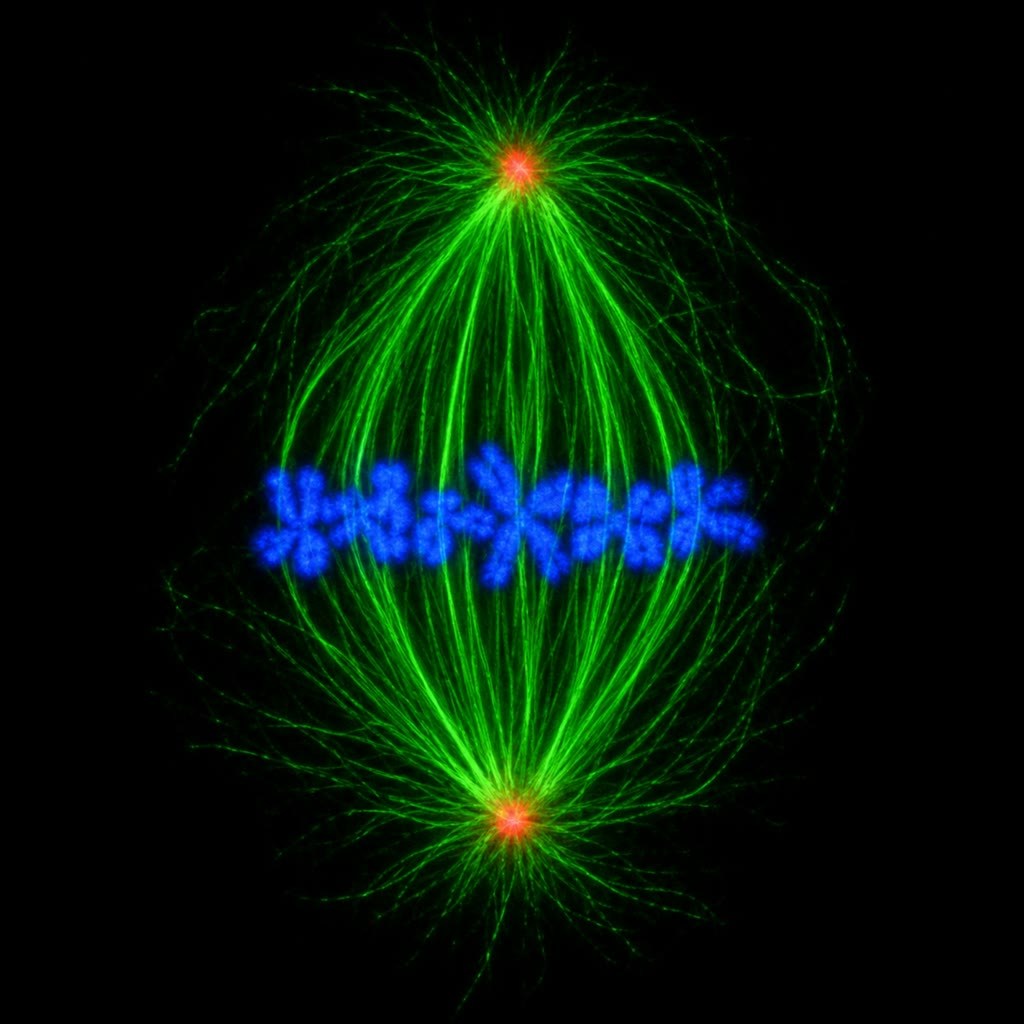
\includegraphics[width=0.36\linewidth]{images/book5/ai/b5-10-mitotic-spindle.jpg}\hspace{0.04\linewidth}
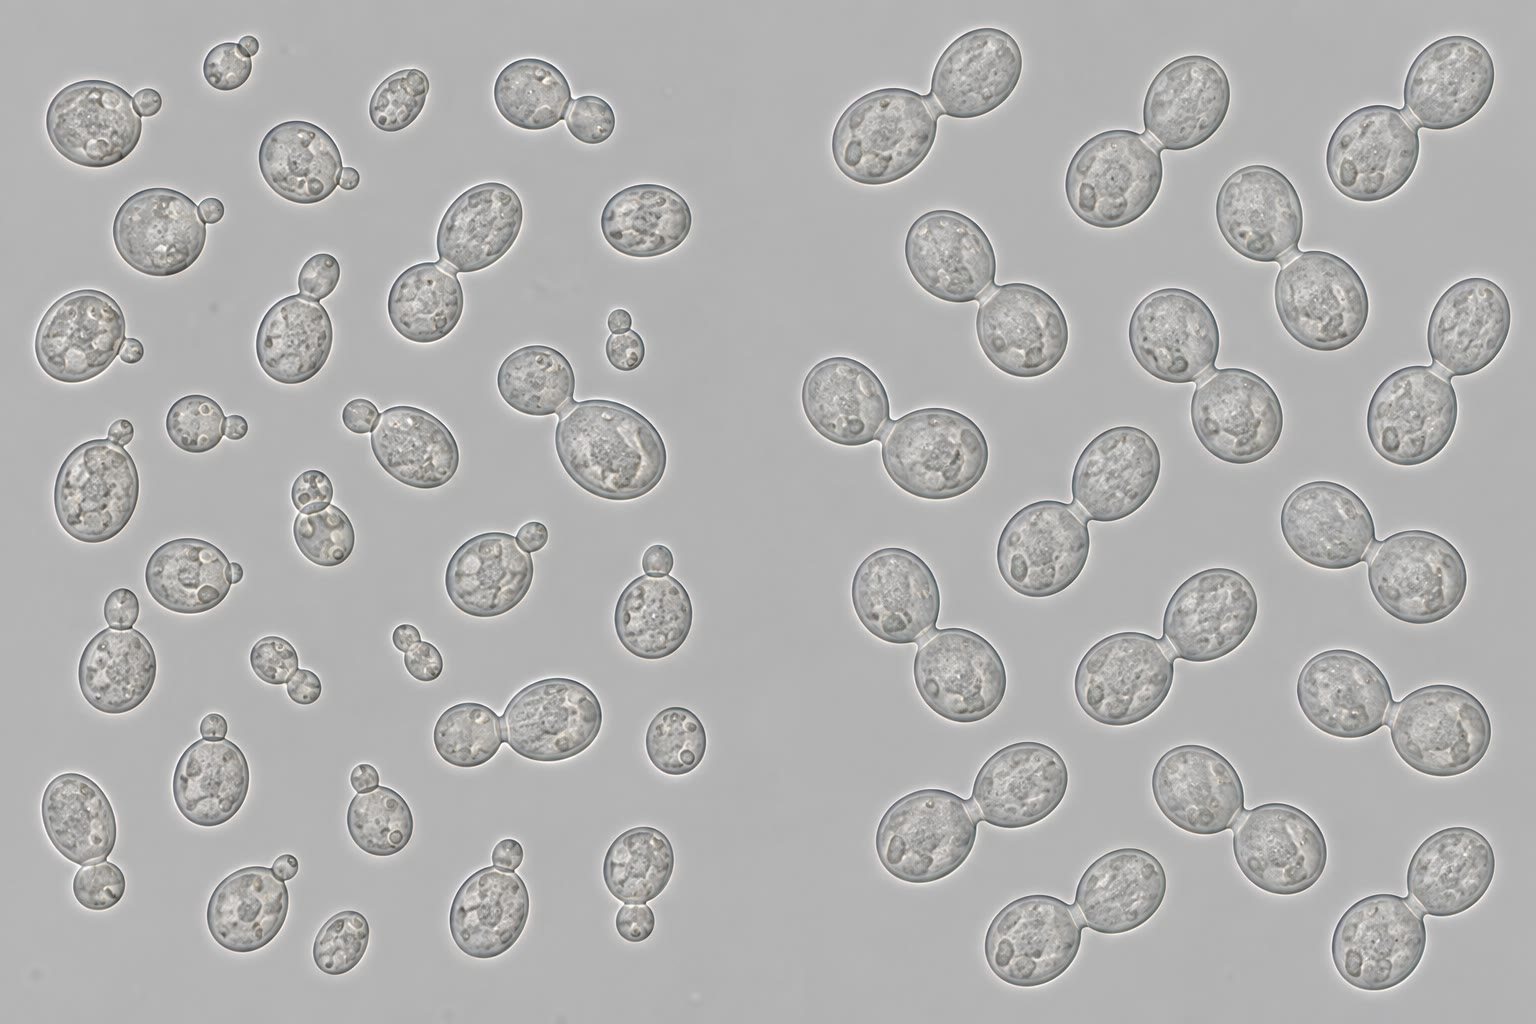
\includegraphics[width=0.54\linewidth]{images/book5/ai/b5-10-yeast-cdc-mutants.jpg}

{\small 左：中期细胞——纺锤体\omterm{def:b3:cytoskeleton-motility:filaments}{微管}（绿色）自
两极（红色）发出，染色体（蓝色）排列在赤道板上，此
时正是纺锤体\omterm{def:b3:cell-cycle-apoptosis:checkpoints}{检查点}作出判定的时刻。右：出芽酵母，
野生型，芽的大小各不相同（左），以及 \emph{cdc} 突变体，
其中所有细胞都停滞在同一阶段，每个细胞都带有大小相同的芽
（右）。}
\end{omfigure}

\section{细胞凋亡}

\begin{definition}[细胞凋亡]\label{def:b3:cell-cycle-apoptosis:apoptosis}
\index{细胞凋亡}\index{坏死}\index{胱天蛋白酶}\index{磷脂酰丝氨酸}
\emph{细胞凋亡}是由内源性程序引发的程序性细胞死亡：细胞
皱缩变圆，其\omterm{def:b3:chromatin-epigenetics:nucleosome}{染色质}凝缩，DNA 在\omterm{def:b3:chromatin-epigenetics:nucleosome}{核小体}之间被切断，
切成梯状片段，细胞核破碎，
膜出泡并形成封闭的小泡，磷脂酰丝氨酸出现在
膜的外表面，作为“吃掉我”的信号，而
片段在一小时内被邻近细胞或巨噬细胞吞噬——
不发生泄漏，因此也不引发炎症。它由
\emph{胱天蛋白酶}执行，它们是一类在天冬氨酸之后切割的半胱氨酸蛋白酶，
以无活性酶原的形式合成：\emph{起始型}胱天蛋白酶（8 和 9）
通过在平台上聚集而被激活，它们切割并激活
\emph{执行型}胱天蛋白酶（3 和 7），它们切割数百种
底物——核纤层蛋白、细胞骨架、DNA 切割核酸酶的抑制剂，
以及使磷脂酰丝氨酸留在膜内侧的酶。
相比之下，\emph{坏死}是由\omterm{def:b3:dna-repair:lesions}{损伤}导致的死亡：细胞肿胀，
破裂，内容物外溢，并引发炎症。细胞凋亡
由克尔、威利和柯里于 1972 年命名并描述了其形态；
其基因则在一种线虫中被发现。
\end{definition}

\begin{proof}[证据]
每个 \emph{Caenorhabditis elegans} 雌雄同体个体产生 $1090$ 个
体细胞，其中同样 $131$ 个细胞死亡，每个都在固定的时间和地点死去。
霍维茨及其同事（1980 年代）分离出一些使这些细胞存活的突变体：
\emph{ced-3} 和 \emph{ced-4} 在每次死亡中都是必需的，在它们
缺失时，$131$ 个细胞存活并分化；\emph{ced-9}
起保护作用——其缺失会杀死本应存活的细胞，其
过度活化则拯救了本应死亡的细胞；\emph{egl-1} 是
某些特定死亡所必需的。CED-3 是一种\omterm{def:b3:cell-cycle-apoptosis:apoptosis}{胱天蛋白酶}，CED-4 是其
激活平台（人类中为 Apaf-1），CED-9 是一种 Bcl-2 蛋白，EGL-1 是一种
仅含 BH3 结构域的蛋白。人类通路，基因逐一对应。
人类 \emph{BCL2} 基因本身曾在滤泡性淋巴瘤的一次染色体易位中被发现，
这是一种细胞不能死亡的癌症。
\end{proof}

\begin{definition}[两条通路]\label{def:b3:cell-cycle-apoptosis:pathways}
\index{内源性通路}\index{外源性通路}\index{Bcl-2 家族}\index{细胞色素 c}\index{凋亡小体}\index{死亡受体}
\emph{内源性}（线粒体）通路整合细胞的
内部状态。\emph{Bcl-2 家族}包括三类：守护者
（Bcl-2、Bcl-xL、Mcl-1），位于线粒体外膜上并
使其保持封闭；效应蛋白（Bax、Bak）激活后寡聚化，
在该膜上形成孔道；以及\emph{仅含 BH3 结构域}的感受器（Bim、Bid、
Puma、Noxa、Bad），各自由特定的\omterm{def:b3:dna-repair:lesions}{损伤}诱导或激活——
通过 \omterm{def:b3:dna-repair:ddr}{p53} 介导的 DNA \omterm{def:b3:dna-repair:lesions}{损伤}（Puma、Noxa）、生长因子撤除（Bim、
Bad）、脱离附着、未折叠蛋白——它们结合守护者并
释放或激活效应蛋白。当效应蛋白占上风时，外膜
被通透化，\emph{细胞色素~c}漏入细胞溶胶，
与 Apaf-1 结合并形成\emph{凋亡小体}，后者激活\omterm{def:b3:cell-cycle-apoptosis:apoptosis}{胱天蛋白酶}~9。
\emph{外源性}通路从外部启动：\emph{死亡受体}（Fas、
TNF 受体、TRAIL 受体）被杀伤性淋巴细胞
或邻近细胞上的配体结合并聚集，招募接头蛋白，并激活
\omterm{def:b3:cell-cycle-apoptosis:apoptosis}{胱天蛋白酶}~8，后者直接切割\omterm{def:b3:cell-cycle-apoptosis:apoptosis}{胱天蛋白酶}~3，并通过 Bid
也开启线粒体通路。两条通路汇聚于
执行型\omterm{def:b3:cell-cycle-apoptosis:apoptosis}{胱天蛋白酶}；抑制蛋白（IAPs、FLIP）
沿途设定阈值。
\end{definition}

\begin{omfigure}
\begin{tikzpicture}[every node/.style={font=\scriptsize}, >=stealth]
  % extrinsic
  \node[draw, thick, rounded corners, fill=omProp!25, align=center] (lig) at (0,4.2) {杀伤细胞上的死亡配体 \\(FasL、TNF、TRAIL)};
  \node[draw, thick, rounded corners, fill=omProp!25, align=center] (rec) at (0,2.8) {死亡受体聚集；\\接头蛋白招募胱天蛋白酶-8};
  \node[draw, thick, rounded corners, fill=omThm!20] (c8) at (0,1.5) {胱天蛋白酶-8 激活};
  % intrinsic
  \node[draw, thick, rounded corners, fill=omDef!20, align=center] (insult) at (7.2,4.2) {DNA 损伤（p53）、生长因子缺失，\\脱离附着、未折叠蛋白};
  \node[draw, thick, rounded corners, fill=omDef!20, align=center] (bh3) at (7.2,3.0) {仅含 BH3 结构域的感受器（Puma、Bim、Bid）\\中和 Bcl-2，激活 Bax/Bak};
  \node[draw, thick, rounded corners, fill=omDef!20, align=center] (mito) at (7.2,1.7) {线粒体外膜打开：\\细胞色素 $c$ 释出，凋亡小体形成};
  \node[draw, thick, rounded corners, fill=omThm!20] (c9) at (7.2,0.5) {胱天蛋白酶-9 激活};
  % convergence
  \node[draw, thick, rounded corners, fill=omThm!35, align=center] (c3) at (3.6,-0.8) {执行型胱天蛋白酶 3 和 7：\\切割数百种底物};
  \node[draw, thick, rounded corners, fill=gray!15, align=center] (out) at (3.6,-2.3) {染色质凝缩，DNA 成梯状，膜出泡，\\磷脂酰丝氨酸外露，被吞噬};
  \draw[->, thick] (lig) -- (rec); \draw[->, thick] (rec) -- (c8); \draw[->, thick] (c8) -- (c3);
  \draw[->, thick] (insult) -- (bh3); \draw[->, thick] (bh3) -- (mito); \draw[->, thick] (mito) -- (c9); \draw[->, thick] (c9) -- (c3);
  \draw[->, thick] (c3) -- (out);
  \draw[->, thick, dashed] (c8) -- (bh3) node[pos=0.55, below, sloped] {Bid 被切割：两条通路汇合};
  \node[left, omThm, align=right] at (-2.3,1.5) {外源性 \\通路}; \node[right, omDef, align=left] at (10.4,1.7) {内源性 \\通路};
  \node[right, font=\tiny, align=left] at (8.6,0.5) {IAPs 在此抑制；\\Bcl-2 在上方守护};
\end{tikzpicture}

{\small 通往执行型\omterm{def:b3:cell-cycle-apoptosis:apoptosis}{胱天蛋白酶}的两条路径。由外向内，\omterm{def:b3:cell-cycle-apoptosis:pathways}{死亡受体}激活胱天蛋白酶-8；
由内向外，Bcl-2 家族权衡细胞的状态，当效应者占上风时，
线粒体释放细胞色素~$c$，胱天蛋白酶-9 被激活。
两者最终都汇聚于胱天蛋白酶-3。}
\end{omfigure}

\begin{proposition}[不可逆的临界点]\label{prop:b3:cell-cycle-apoptosis:mompt}
\index{线粒体外膜通透化}
线粒体外膜的通透化是突然发生的——
同一细胞内的所有线粒体都在约五分钟内开放，
此前却经历数小时的“权衡”——并且是彻底的：一旦细胞色素~$c$
进入细胞质，\omterm{def:b3:cell-cycle-apoptosis:apoptosis}{胱天蛋白酶}随之在数分钟内被激活，且撤除刺激也无法使之逆转。
有两个特征使其成为开关。
Bax/Bak 孔道通过寡聚化形成，因此其速率随激活的效应者数量急剧上升；
而守护者与感受者以高亲和力相互结合，
于是在达到阈值之前，每个感受者都被中和，
越过阈值之后，每多出一个感受者便是游离的——这是一种滴定，好比缓冲液被耗尽。
因此细胞并非逐渐死亡，
而是不断积累仅含 BH3 的蛋白，直至越过阈值，
随即一并死亡。模拟 BH3 蛋白的药物（维奈托克，占据 Bcl-2）
能将“已致敏”的细胞——即已接近阈值的细胞，许多白血病细胞正是如此——
推过阈值，
而不影响未致敏的细胞。
\end{proposition}

\begin{omfigure}
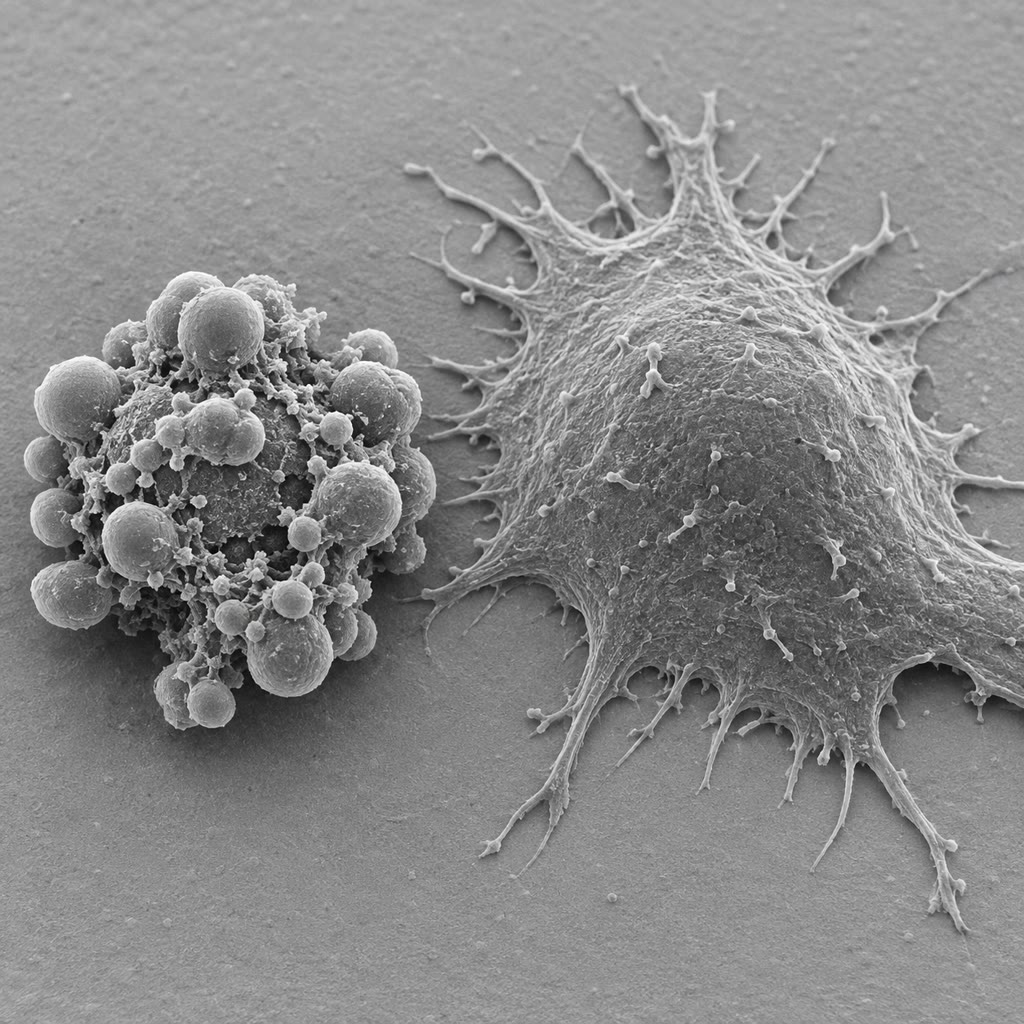
\includegraphics[width=0.40\linewidth]{images/book5/ai/b5-10-apoptotic-cell.jpg}

{\small 扫描电子显微镜下，凋亡细胞与一个健康细胞并排：细胞皱缩，
表面碎裂成封闭的泡状突起，这些突起将被吞噬，
不留任何炎症痕迹。}
\end{omfigure}

\begin{example}[建造身体的死亡]\label{ex:b3:cell-cycle-apoptosis:development}
手指是由手掌状的原基经\omterm{def:b3:cell-cycle-apoptosis:apoptosis}{细胞凋亡}雕刻而成的，
其间的细胞被清除；在鸭子中，这些细胞却存活下来，蹼便保留了下来。
蝌蚪的尾巴在变态时，
在甲状腺激素的信号下被吸收。脊椎动物神经系统中约有一半产生的神经元在出生前死亡，
即那些未能从靶细胞获得足够营养因子的神经元——
这一竞争使神经元的数量与其所服务的区域大小相匹配。
胸腺中产生的 T 细胞有 95\%在那里死亡，
因为它们不识别任何东西，或识别自身，因而被筛选淘汰
（见\cref{ch:b3:adaptive-immunity}）。
每天，肠上皮在绒毛顶端脱落其最老的细胞，皮肤脱落角质形成细胞，
血液中的\omterm{def:b3:cell-cycle-apoptosis:other}{衰老}中性粒细胞则在存活一天后被清除：\omterm{def:b3:cell-cycle-apoptosis:apoptosis}{细胞凋亡}是日常的常规过程，
而组织的大小
取决于两个较大速率之间的差值。
\end{example}

\section{其他的退出方式，以及退出失败}

\begin{definition}[调控性坏死与衰老]\label{def:b3:cell-cycle-apoptosis:other}
\index{坏死性凋亡}\index{细胞焦亡}\index{衰老}
细胞还有其他程序性死亡方式，凡\omterm{def:b3:cell-cycle-apoptosis:apoptosis}{细胞凋亡}无声无息之处，它们都伴有炎症。
\emph{\omterm{def:b3:cell-cycle-apoptosis:apoptosis}{坏死}性凋亡}在胱天蛋白酶-8 被阻断时由\omterm{def:b3:cell-cycle-apoptosis:pathways}{死亡受体}触发
（某些病毒正是这样阻断它），它将激酶 RIPK3 与 MLKL \omterm{def:b3:genomics:assembly}{组装}在一起，
使质膜穿孔。\emph{细胞焦亡}发生于受感染的巨噬细胞中，
由炎症小体的胱天蛋白酶-1 执行（见\cref{ch:b3:innate-immunity}），
该酶切割 gasdermin，使其形成成孔蛋白，
并释放白细胞介素-1。\emph{铁死亡}是一种依赖铁的脂质过氧化所致的死亡。
细胞也可以停止分裂而不死亡：\emph{衰老}是一种永久性的停滞，
在端粒磨损（见\cref{ch:b3:stem-cells}）、\omterm{def:b3:cytoskeleton-motility:motors}{持续性} DNA \omterm{def:b3:dna-repair:lesions}{损伤}或癌基因激活之后，
由 p16 和 p21 强制施加；
处于衰老状态的细胞代谢上仍然活跃，并分泌炎症因子。
衰老使受损细胞退出分裂群体——
这是一种肿瘤抑制机制——
并随年龄增长而累积，
其分泌物促成组织的退化；在小鼠中清除衰老细胞可延长健康寿命。
\end{definition}

\begin{remark}[过少与过多]\label{rem:b3:cell-cycle-apoptosis:disease}
这些程序的疾病与剂量有关。死亡过少：
癌症，其中凋亡阈值因 Bcl-2 过表达或 \omterm{def:b3:dna-repair:ddr}{p53} 丢失而升高，
使带有受损基因组的细胞得以存活，并积累更多\omterm{def:b3:dna-repair:lesions}{损伤}；
自身免疫，即本应在选择中死亡的淋巴细胞持续存活。死亡过多：
HIV 感染中 T 细胞的丧失；
脑卒中半影区的神经元在缺血数小时后通过\omterm{def:b3:cell-cycle-apoptosis:apoptosis}{细胞凋亡}死亡
（这是一个治疗窗口）；神经退行性疾病中神经元的缓慢凋亡；
心脏病发作后心肌细胞的丧失。
癌症治疗在很大程度上是有意诱导阈值
低于邻近细胞的细胞发生凋亡；
而针对 Bcl-2 和 Cdk4/6 的药物，
是首批依据本章所述图谱设计的药物。
\end{remark}

\section{练习}

\begin{exercise}[$\star$]\label{exo:b3:cell-cycle-apoptosis:1}
列出\omterm{def:b3:cell-cycle-apoptosis:cdk}{细胞周期}的四个时期，驱动各转换的周期蛋白--CDK 对，
以及结束有丝分裂的泛素连接酶。
\end{exercise}

\begin{exercise}[$\star$]\label{exo:b3:cell-cycle-apoptosis:2}
Hartwell、Nurse 和 Hunt 各自对发现这一“引擎”做出了什么贡献，
分别使用的是哪种生物？
\end{exercise}

\begin{exercise}[$\star$]\label{exo:b3:cell-cycle-apoptosis:3}
说出三个\omterm{def:b3:cell-cycle-apoptosis:checkpoints}{检查点}、各自检测的条件，以及
各自作用的分子靶点。
\end{exercise}

\begin{exercise}[$\star$]\label{exo:b3:cell-cycle-apoptosis:4}
从五个特征上区分\omterm{def:b3:cell-cycle-apoptosis:apoptosis}{细胞凋亡}与\omterm{def:b3:cell-cycle-apoptosis:apoptosis}{坏死}，
并说出执行\omterm{def:b3:cell-cycle-apoptosis:apoptosis}{细胞凋亡}的酶的类别。
\end{exercise}

\begin{exercise}[$\star\star$]\label{exo:b3:cell-cycle-apoptosis:5}
在蛙卵提取物中，周期蛋白 B 以 $k_{s} = 1$ 单位每分钟合成；
有丝分裂阈值为 $C_{2} = 30$ 单位，退出阈值为 $C_{1} = 5$，
并且在有丝分裂中，周期蛋白以半衰期
\qty{2}{min} 降解。估算振荡的周期，以及
\omterm{def:b3:cell-cycle-apoptosis:cdk}{细胞周期}中处于有丝分裂的时间所占的比例。
\end{exercise}

\begin{exercise}[$\star\star$]\label{exo:b3:cell-cycle-apoptosis:6}
预测一个细胞在下列情形下的行为：（a）表达
不可降解的周期蛋白 B；（b）缺失 Wee1；（c）缺失 Cdc25；（d）表达
一种不能被 Wee1 磷酸化的 Cdk1，依据
\cref{thm:b3:cell-cycle-apoptosis:oscillator}中的振子加以说明。
\end{exercise}

\begin{exercise}[$\star\star$]\label{exo:b3:cell-cycle-apoptosis:7}
一次 Rao--Johnson 融合将一个 G1 期细胞与一个 S 期细胞相融合；另一次
则将一个 G2 期细胞与一个 S 期细胞相融合。预测每个细胞核会发生什么变化，并
借助\omterm{def:b3:cell-cycle-apoptosis:checkpoints}{复制许可}和 CDK 水平加以解释。
\end{exercise}

\begin{exercise}[$\star\star$]\label{exo:b3:cell-cycle-apoptosis:8}
解释为何单个未附着的动粒能使整个细胞的
后期停滞，并预测 Mad2 缺失的细胞的
命运。
\end{exercise}

\begin{exercise}[$\star\star$]\label{exo:b3:cell-cycle-apoptosis:9}
预测缺失 \emph{ced-9} 的线虫、缺失
\emph{ced-3} 的线虫，以及两者均缺失的线虫，依据该通路
解释上位性。
\end{exercise}

\begin{exercise}[$\star\star\star$]\label{exo:b3:cell-cycle-apoptosis:10}
证明：不含双稳态开关、仅有一条负反馈环的系统
——周期蛋白以 $k_{s}$ 合成，以 $k_{d}AC$ 降解，其中 $A$
与 $C$ 成简单正比——具有稳定的稳态，且不发生
振荡。S 形曲线增加了什么，若代之以延迟，
又会增加什么？
\end{exercise}

\begin{exercise}[$\star\star\star$]\label{exo:b3:cell-cycle-apoptosis:11}
某细胞含有 $N$ 个守护者 Bcl-2 分子，并在受\omterm{def:b3:dna-repair:lesions}{损伤}刺激后接收仅含 BH3 的
感受器，速率为每小时 $r$ 个，每个感受器
结合一个守护者。解释为何细胞大约在时刻 $N/r$ 死亡，
无论此后刺激强度多大，为何死亡是突然发生的，
以及维奈托克拉对该时间有何影响。
\end{exercise}

\begin{exercise}[$\star\star\star$]\label{exo:b3:cell-cycle-apoptosis:12}
滤泡性淋巴瘤携带一个使
\emph{BCL2} 过表达的易位，其细胞分裂缓慢；视网膜母细胞瘤携带
\emph{RB} 缺失，其细胞分裂迅速。解释每一种单一\omterm{def:b3:dna-repair:lesions}{损伤}如何
导致肿瘤形成，为何前者惰性而后者侵袭性强，
并说明二者分别反映了本章中的哪两类程序。
\end{exercise}

\section{问题：上皮的生与死}

\begin{problem}[{周末问题——肠道内衬逐细胞更新，
细胞周期由周期蛋白振子计时，检查点的错误
在全身范围内计数，并称量每天凋亡清除的
一千亿个细胞的质量，最后求周期长度、
每天产生的非整倍性细胞数，以及身体经细胞凋亡回收的
质量}]
\label{pb:b3:cell-cycle-apoptosis:1}
已知：小肠有 $10^{7}$ 个隐窝，每个隐窝更新一条
含 \num{3500} 个细胞的绒毛，每 $5$ 天一次；每个隐窝约有 $22$ 个干细胞，
每天分裂一次，其子代在分化之前还要再分裂
$5$ 次。振子：周期蛋白合成速率 $k_{s} = 2$ 单位每小时，
$C_{2} = 40$ 单位，$C_{1} = 8$，有丝分裂周期蛋白的半衰期
\qty{10}{min}。\omterm{def:b3:cell-cycle-apoptosis:checkpoints}{检查点}：若无纺锤体\omterm{def:b3:cell-cycle-apoptosis:checkpoints}{检查点}，每
$50$ 次分裂中有一次染色体错分离；有该\omterm{def:b3:cell-cycle-apoptosis:checkpoints}{检查点}时，每 \num{50000} 次中才有一次。身体
每天更替 $10^{11}$ 个细胞，每个细胞质量 \qty{1}{ng}，蛋白质占
质量的 \qty{20}{\%}；一个巨噬细胞清除一个凋亡细胞所需的时间为
\qty{1}{h}。

\medskip
\noindent\textbf{第一部分——更新。}
\begin{enumerate}
  \item 小肠每天脱落多少个细胞，每
        秒脱落多少个？
  \item 一个隐窝每天产生多少个细胞？核对：$22$ 次
        干细胞分裂，每个定向子代还要再分裂 $5$
        次。
  \item 若一个干细胞每天分裂一次，寿命为 $80$ 年，
        共分裂多少次？若每个基因组每次分裂的突变率为 $0.6$
        （见\cref{ch:b3:dna-repair}），则它会
        积累多少个突变？
  \item 过渡细胞每 \qty{12}{h} 分裂一次。为何组织能够
        负担快速、短寿的过渡分裂，却让干细胞
        保持缓慢？
  \item 一次辐射剂量杀死所有分裂中的过渡细胞，但
        保留干细胞，它们在一天内即恢复分裂。
        绒毛得不到补充，多久后会裸露，重建它又需
        多久？为何肠道是辐射的早期受害者？
  \item 在结肠中，顶端的脱落通过\omterm{def:b3:cell-cycle-apoptosis:apoptosis}{细胞凋亡}实现（失巢凋亡，
        即脱离附着后的死亡）。为何对于一个
        与肠道细菌接触的细胞，这是正确的死亡方式？
\end{enumerate}

\medskip
\noindent\textbf{第二部分——时钟。}
\begin{enumerate}[resume]
  \item 由振子数据可知，周期蛋白从 $C_{1}$
        升至 $C_{2}$ 需要多长时间？
  \item 有丝分裂降解使其从 $C_{2}$
        回落至 $C_{1}$ 需要多长时间？
  \item 裸振子的周期，以及 Cdk1 处于活性状态
        所占周期的比例。
  \item 隐窝中的过渡\omterm{def:b3:cell-cycle-apoptosis:cdk}{细胞周期}为 \qty{12}{h}，干\omterm{def:b3:cell-cycle-apoptosis:cdk}{细胞
        周期}为 \qty{24}{h}，蛙卵为 \qty{30}{min}。模型的
        哪个参数不同，以及在体细胞中是什么
        提供了这一差异？
  \item 一个因 DNA \omterm{def:b3:dna-repair:lesions}{损伤}而停滞于 G2/M \omterm{def:b3:cell-cycle-apoptosis:checkpoints}{检查点}的细胞
        仍在合成周期蛋白 B。它在相平面上位于何处，以及
        是什么使它保持在那里？\omterm{def:b3:dna-repair:lesions}{损伤}修复后会发生什么？
  \item 一种药物抑制 APC/C。描述在其存在下进入
        有丝分裂的细胞的命运。
\end{enumerate}

\medskip
\noindent\textbf{第三部分——错误。}
\begin{enumerate}[resume]
  \item 身体每天要进行多少次分裂，
        才能替换 $10^{11}$ 个细胞？
  \item 有\omterm{def:b3:cell-cycle-apoptosis:checkpoints}{检查点}时与无\omterm{def:b3:cell-cycle-apoptosis:checkpoints}{检查点}时，每天分别
        产生多少个非整倍性子代细胞？
  \item 大多数非整倍性细胞会死亡或停滞（\omterm{def:b3:dna-repair:ddr}{p53} 对错误分离
        作出反应）。若 \qty{1}{\%} 存活并继续分裂，
        则具有\omterm{def:b3:cell-cycle-apoptosis:checkpoints}{检查点}功能的身体每天产生多少个正在分裂的非整倍性细胞，
        一生中又产生多少个？
  \item 一个含 $10^{9}$ 个细胞的肿瘤丧失了\omterm{def:b3:cell-cycle-apoptosis:checkpoints}{检查点}和 \omterm{def:b3:dna-repair:ddr}{p53}。
        它每天发生多少次错误分离，为什么这使它
        演化得很快？
  \item 解释为什么纺锤体\omterm{def:b3:cell-cycle-apoptosis:checkpoints}{检查点}完全丧失对胚胎是致命的，
        而部分丧失却会促进癌症。
  \item 唐氏综合征源于减数分裂而非有丝分裂中的错误分离。
        解释为什么该处某一个细胞的错误会影响患儿的每一个细胞，
        而一次有丝分裂错误只影响一个细胞系。
\end{enumerate}

\medskip
\noindent\textbf{第四部分——清除。}
\begin{enumerate}[resume]
  \item 身体每天通过\omterm{def:b3:cell-cycle-apoptosis:apoptosis}{细胞凋亡}清除多少质量的细胞，
        每年又是多少？与体重相比如何？
  \item 每天相当于多少蛋白质？以膳食摄入量作参照，
        每日 \qty{70}{g} 的摄入量相比，身体蛋白质更新中
        死亡细胞的回收占多大比例？
  \item 每天死亡的细胞需要多少个持续工作的巨噬细胞才能清除？
        身体约有 $10^{11}$ 个巨噬细胞，
        它们的工作时间占比是多少？
  \item 为什么尸体必须在裂解之前被清除，
        什么信号表示“吃我”？
  \item 某患者的 B~细胞中 Bcl-2 过表达。哪条途径被阻断，
        外源性途径是否仍然有效，
        结果为何是缓慢生长的淋巴瘤而非快速生长的淋巴瘤？
  \item 脑卒中半影区的神经元在\omterm{def:b3:dna-repair:lesions}{损伤}后六至
        二十四小时通过\omterm{def:b3:cell-cycle-apoptosis:apoptosis}{细胞凋亡}死亡，核心区的神经元则
        在数分钟内通过\omterm{def:b3:cell-cycle-apoptosis:apoptosis}{坏死}死亡。为什么前者为治疗提供了时间窗口，
        而后者没有？
  \item 总结：裸振子的周期（第~9~题）、
        正常身体中每天正在分裂的非整倍性细胞数
        （第~15~题），以及每天通过\omterm{def:b3:cell-cycle-apoptosis:apoptosis}{细胞凋亡}回收的质量
        （第~19~题）。
\end{enumerate}
\end{problem}
